\label{sec:evaluation}

\begin{figure*}[!t]
{\centering
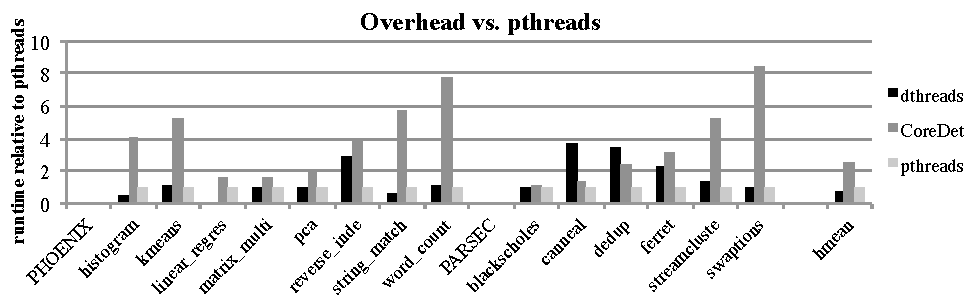
\includegraphics[width=5in]{dthreads/figure/overhead-figure}
\caption{Normalized execution time with respect to \pthreads{} (lower is better). For 9 of the 14 benchmarks, \dthreads{} runs nearly as fast or faster than \pthreads{}, while providing deterministic behavior.\label{fig:performance}}
}
\end{figure*}



We perform our evaluation on an Intel Core 2 dual-processor CPU system
equipped with 16GB of RAM. Each processor is a 4-core 64-bit Xeon
running on at 2.33GHZ with a 4MB L2 cache.  The operating system is an
unmodified CentOS 5.5, running with Linux kernel version
2.6.18-194.17.1.el5.

\subsection{Methodology}

We evaluate the performance and scalability of \dthreads{} versus
CoreDet and \pthreads{} across the PARSEC~\cite{parsec} and
Phoenix~\cite{phoenix-hpca} benchmark suites.  We do not include
results for \texttt{bodytrack}, \texttt{fluidanimate}, \texttt{x.264},
\texttt{facesim}, \texttt{vips}, and \texttt{raytrace} benchmarks from PARSEC, 
since they do not currently work with \dthreads{} (note that many of
these also do not work for CoreDet).

In order to compare performance directly against CoreDet, which relies
on the LLVM infrastructure~\cite{LLVM:CGO04}, all benchmarks are
compiled with the LLVM compiler at the ``-O5'' optimization
level~\cite{LLVM:CGO04}. Since \dthreads{} does not currently support
64-bit binaries, all benchmarks are compiled for 32 bit environments
(using the ``-m32'' compiler flag). Each benchmark is executed ten
times on a quiescent machine. To reduce the effect of outliers, the
lowest and highest execution times for each benchmark are discarded,
so each result represents the average of the remaining eight runs.

\textbf{Tuning CoreDet: } 
The performance of CoreDet~\cite{Bergan:2010:CCR:1736020.1736029} is
extremely sensitive to three parameters: the granularity for the
ownership table (in bytes), the quantum size (in number of
instructions retired), and the choice between full serial mode and
reduced serial mode. We compare the performance and scalability
of \dthreads{} with the best possible results that we could obtain for
CoreDet on our system---that is, with the lowest average normalized
runtimes---after an extensive search of the parameter space (six
possible granularities and 8 possible quanta, for each benchmark). The
results presented here are for a 64-byte granularity and a quantum
size of 100,000 instructions, in full serial mode.
 
For all scalability experiments, we logically disable CPUs using
Linux's CPU hotplug mechanism, which allows us to disable or enable
individual CPUs by writing ``0'' (or ``1'') to a special pseudo-file
(\texttt{/sys/devices/system/cpu/cpuN/online}).

\subsection{Determinism}

We first experimentally verify \dthreads{}' ability to ensure
determinism by executing the \emph{racey} determinism
tester~\cite{1508256}. This stress test contains, as its name
suggests, numerous data races and is thus extremely sensitive to
memory-level non-determinism. \dthreads{} reports the same results for
2,000 runs.

\subsection{Performance}
\label{sec:performance}

We next compare the performance of \dthreads{} to CoreDet
and \pthreads{}. Figure~\ref{fig:performance} presents these results
graphically (normalized to \pthreads{}); Table~\ref{tbl:benchmarks}
provides detailed numbers.

\dthreads{} outperforms CoreDet on 12 out
of 14 benchmarks (running between 20\% and $11.2\times$ faster), while
for 9 benchmarks, \dthreads{} provides nearly the same as or higher
performance than \texttt{pthreads}. Because \dthreads{} isolates
updates in separate processes, it can improve performance by
eliminating false sharing---since concurrent ``threads'' actually
execute in different address spaces, there is no coherence traffic
between synchronization points. \dthreads{} eliminates catastrophic
false sharing in the \texttt{linear\_regression} benchmark, allowing
it to execute over $7\times$ faster than \pthreads{} and $11\times$
faster than CoreDet. The \texttt{string\_match} benchmark exhibits a
similar, though less dramatic, false sharing problem,
allowing \dthreads{} to run almost 60\% faster than \pthreads{} and
$9\times$ faster than CoreDet. Two benchmarks, \texttt{histogram}
and \texttt{swaptions}, also run faster with \dthreads{} than
with \pthreads{} ($2\times$ and $6\%$, respectively; $2.7\times$ and
$9\times$ faster than with CoreDet). We believe but have not yet
verified that the reason is false sharing.

For some benchmarks, \dthreads{} incurs modest overhead. For example,
unlike most benchmarks examined here, which create long-lived threads,
the
\texttt{kmeans} benchmark creates and destroys over 1,000 threads in the course of its execution. 
While Linux processes are relatively lightweight, creating and tearing
down a process is still more expensive than the same operations for
threads, accounting for a 14\% performance degradation of \dthreads{}
over \pthreads{} (though it runs $4.6\times$ faster than CoreDet).

\dthreads{} runs substantially slower than \pthreads{} for 4 of the 14
benchmarks examined here. The \texttt{ferret} benchmark relies on an
external library to analyze image files during the first stage in its
pipelined execution model; this library makes intensive (and in the
case of \dthreads{}, unnecessary) use of locks. Lock acquisition and
release in \dthreads{} imposes higher overhead than
ordinary \pthreads{} mutex operations. More importantly in this case,
the intensive use of locks in one stage forces \dthreads{} to
effectively serialize the other stages in the pipeline, which must
repeatedly wait on these locks to enforce a deterministic lock
acquisition order. The other three benchmarks
(\texttt{canneal}, \texttt{dedup}, and \texttt{reverse\_index}) modify
a large number of pages. With \dthreads{}, each page modification
triggers a segmentation violation, a system call to change memory
protection, the creation of a private copy of the page, and a
subsequent copy into the shared space on commit (see
Section~\ref{sec:future-work} for planned optimizations that may
reduce this cost). We note that CoreDet also substantially degrades
performance for these benchmarks, so much of this slowdown may be
inherent to any deterministic runtime system.

\subsection{Scalability}
\label{sec:scalability}

\begin{figure}
{\centering
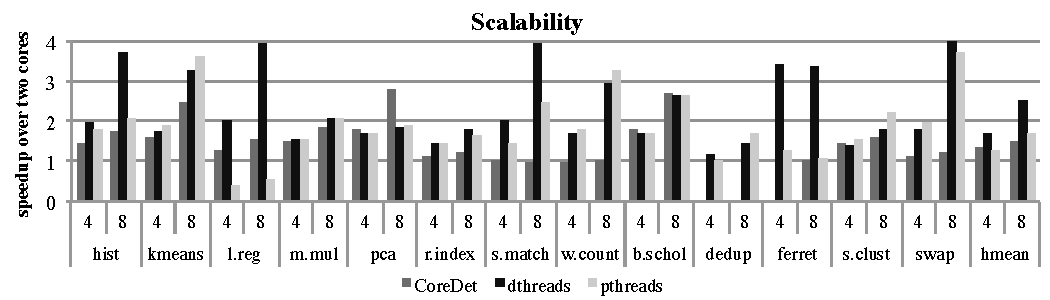
\includegraphics[width=6in]{dthreads/figure/scalability-figure}
\caption{Speedup of eight cores versus two cores (higher is better).  When possible to control with command line options, the number of threads was matched to the number of cores enabled.\label{fig:scalability}}
}
\end{figure}

To measure the scalability cost of running \dthreads{}, we ran two benchmark suite (excluding \texttt{canneal}) on the same machine with eight cores and again with two cores enabled.  Whenever possible without source code modifications, the number of threads was matched to the number of CPUs enabled.  We have found that \dthreads{} scales at least as well as \pthreads{} for 9 of 13 benchmarks, and scales as well or better than CoreDet for all but one benchmark where \dthreads{} outperforms CoreDet by 2x.  Detailed results of this experiment are presented in Figure~\ref{fig:scalability} and discussed below.

\texttt{canneal} was excluded from the scalability experiment because this benchmark does more work when more threads are present, making the performance comparison between eight and two threads unfair.  \dthreads{} hurts scalability relative to \pthreads{} for four of the benchmarks: \texttt{kmeans}, \texttt{word\_count}, \texttt{dedup}, and \texttt{streamcluster} although only marginally in most cases.  In all of these cases, \dthreads{} scales better than CoreDet.

\dthreads{} is able to match the scalability of \pthreads{} for three benchmarks: \texttt{matrix\_multiply}, \texttt{pca}, and \texttt{blackscholes}.  With \dthreads{}, scalability actually \emph{improves} over \pthreads{} for 6 out of 13 benchmarks: \texttt{histogram}, \texttt{linear\_regression}, \texttt{reverse\_index}, \texttt{string\_match}, \texttt{ferret}, and \texttt{swaptions}.




\subsection{Performance Analysis}

The data presented in Table~\ref{tbl:characteristics} are obtained
from the executions running on all 8 cores.  Column 2 shows the
percentage of time spent in the serial phase.  In \dthreads{}, all
memory commits and actual synchronization operations are performed in
the serial phase.  The percentage of time spent in the serial phase
thus can affect performance and scalability. Applications with higher
overhead in \dthreads{} often spend a higher percentage of time in the
serial phase, primarily because they modify a large number of pages
that are committed during that phase.

Column 3 shows the number of transactions in each application and
Column 4 provides the average length of each transaction (ms).  Every
synchronization operation, including locks, conditional variable,
barriers, and thread exits, demarcate transaction boundaries
in \dthreads{}.  For
example, \texttt{reverse\_index}, \texttt{dedup}, \texttt{ferret}
and \texttt{streamcluster} perform numerous transactions whose
execution time is less than 1ms, imposing a performance penalty for
these applications.  Benchmarks with longer (or fewer) transactions run
almost the same speed as or faster than \texttt{pthreads},
including \texttt{histogram} or \texttt{pca}.  In \dthreads{}, longer
transactions amortize the overhead of memory protection and copying.

Column 5 and 6 provides more detail on the costs associated with
memory updates (the number and total volume of dirtied pages). From
the table, it becomes clear why \texttt{canneal} (the most notable
outlier) runs much slower with \dthreads{} than with \pthreads{}. This benchmark
updates over 3 million pages, leading to the creation of
private copies, protection faults, and commits to the shared memory
space. Copying alone is quite expensive: we found that copying one
gigabyte of memory takes approximately 0.8 seconds when
using \texttt{memcpy}, so for \texttt{canneal}, copying overhead alone
accounts for at least 20 seconds of time spent in \dthreads{} (out of
39s total).

\textbf{Conclusion: }
Most benchmarks examined here contain either a small number or long
running transactions, and modify a modest number of pages during
execution. For these applications, \dthreads{} is able to amortize its
various overheads; by eliminating false sharing, it can even run faster than
\pthreads{}. However, for the few benchmarks that perform numerous short-lived
transactions, or modify a large amount of pages, \dthreads{} can
exhibit substantial overhead.

% The memory overhead of \dthreads{} includes memory
%protection system calls overhead, memory trap overhead and memory
%commit overhead.  Memory overhead of \dthreads{} are based on page
%granularity, capturing those dirty pages using page protection,
%tracking modifications of one thread by diffing private pages with
%twin pages and committing changes to the shared mapping in the end.

\begin{table*}[!t]
\centering
\begin{tabular}{l|rrr|rr|l}
{\bf \small Benchmark} & {\bf \small CoreDet} & {\bf \small \dthreads{}} & {\bf \small \pthreads{}} & $\frac{\mbox{\bf \small CoreDet}}{\mbox{\bf \small \pthreads{}}}$ & $\frac{\mbox{\small \bf \dthreads{}}}{\mbox{\small \bf \pthreads{}}}$ & {\bf \small Input} \\

\hline
{\bf \small histogram} & 0.97 & 0.73 & 0.35 & $1.32\times$ & $0.48\times$ & {\it \small large.bmp} \\
{\bf \small kmeans} & 68.41 & 13.16 & 15.02 & $5.20\times$ & $1.14\times$ & {\it \small -d 3 -c 1000 -p 100000 -s 1000} \\ 
{\bf \small linear\_regression} & 6.42 & 4.11 & 0.57  & $1.56\times$ & $0.14\times$ & {\it \small key\_file\_500MB.txt} \\
{\bf \small matrix\_multiply} & 31.68 & 19.32 & 19.28  & $1.63\times$ & $0.99\times$ & {\it \small 2000 2000 } \\
{\bf \small pca} & 39.24 & 20.49 & 21.14  & $1.92\times$ & $1.03\times$ & {\it \small -r 4000 -c 4000 -s 100 } \\
{\bf \small reverse\_index} & 7.85 & 2.06 & 6.53 & $3.81\times$ & $3.17\times$ & {\it \small datafiles} \\
{\bf \small string\_match} & 18.31 & 3.19 & 1.97 & $5.74\times$ & $0.62\times$ & {\it \small key\_file\_500MB.txt} \\
{\bf \small word\_count} & 17.17 & 2.17 & 2.37 & $7.91\times$ & $1.09\times$ & {\it \small word\_100MB.txt} \\
{\bf \small blackscholes} & 10.49 & 9.47 & 9.30 & $1.11\times$ & $0.98\times$ & {\it \small 8 in\_1M.txt prices.txt} \\
{\bf \small canneal} & 14.74 & 10.41 & 39.82 & $1.42\times$ & $3.83\times$ &  {\it \small 7 15000 2000 400000.nets 128} \\
{\bf \small dedup} & 3.38 & 1.45 & 5.39 & $2.33\times$ & $3.72\times$ & {\it \small -c -p -f -t 2 -i media.dat output.txt} \\
{\bf \small ferret} & 21.89 & 7.02 & 26.86 & $3.11\times$ & $3.83\times$ & {\it \small corel lsh queries 10 20 1 output.txt} \\
{\bf \small streamcluster} & 14.33 & 2.74 & 4.61 & $5.23\times$ & $1.68\times$ &  {\it \small 10 20 128 16384 16384 1000 none output.txt 8} \\
{\bf \small swaptions} & 35.21 & 4.18 & 3.88 & $8.42\times$ & $0.93\times$ & {\it \small -ns 128 -sm 50000 -nt 8} \\
% was dthreads, pthreads, coredet
%{\bf \small histogram} & 0.35 & 0.73 & 0.97 & {\bf \small large.bmp} \\
%{\bf \small kmeans} & 15.02 & 13.16 & 68.41 & {\bf \small -d 3 -c 1000 -p 100000 -s 1000} \\ 
%{\bf \small linear\_regression} & 0.57 & 4.11 & 6.42 &  {\bf \small key\_file\_500MB.txt} \\
%{\bf \small matrix\_multiply} & 19.28 & 19.32 & 31.68 & {\bf \small 2000 2000 } \\
%{\bf \small pca} & 21.14 & 20.49 & 39.24 & {\bf \small -r 4000 -c 4000 -s 100 } \\
%{\bf \small reverse\_index} & 6.53 & 2.06 & 7.85 & {\bf \small datafiles} \\
%{\bf \small string\_match} & 1.97 & 3.19 & 18.31 & {\bf \small key\_file\_500MB.txt} \\
%{\bf \small word\_count} & 2.37 & 2.17 & 17.17 & {\bf \small word\_100MB.txt} \\
%{\bf \small blackscholes} & 9.30 & 9.47 & 10.49 & {\bf \small 8 in\_1M.txt prices.txt} \\
%{\bf \small canneal} & 39.82 & 10.41 & 14.74 & {\bf \small 7 15000 2000 400000.nets 128} \\
%{\bf \small dedup} & 5.39 & 1.45 & 3.38 & {\bf \small -c -p -f -t 2 -i media.dat output.txt} \\
%{\bf \small ferret} & 26.86 & 7.02 & 21.89 & {\bf \small corel lsh queries 10 20 1 output.txt} \\
%{\bf \small streamcluster} & 4.61 & 2.74 & 14.33 & {\bf \small 10 20 128 16384 16384 1000 none output.txt 8} \\
%{\bf \small swaptions} & 3.88 & 4.18 & 35.21 & {\bf \small -ns 128 -sm 50000 -nt 8} \\
\hline
\end{tabular}
\caption{Benchmarks: execution time (in seconds) and input parameters.\label{tbl:benchmarks}}
\end{table*}


\begin{table*}[!t]
\centering
\begin{tabular}{l|rrrrr}
& {\bf \small Serial Phase} & {\bf \small Transactions} & {\bf \small TransLength} & {\bf \small DirtyPages} & {\bf \small DirtyPages}
\\
{\bf \small Benchmark} & {\bf \small (\% of time)} & {\bf (\#)} & {\bf \small (ms)} & {\bf \small (\#)} & {\bf \small (GB)}\\
%\hline
%\multicolumn{6}{|c|}{\emph{Phoenix}} \\
\hline
\small \textbf{histogram} & 0 & 23 & 15.47 & 29 & 0 \\
\small \textbf{kmeans} & 0 & 3929 & 3.82 & 9466 & 0.04\\
\small \textbf{linear\_regression} & 0 & 24 & 23.92 & 17 & 0\\
\small \textbf{matrix\_multiply} & 0 & 24 & 841.2 & 3945 & 0.02\\
\small \textbf{pca} & 0 & 48 & 443 & 11471 & 0.04 \\
\small \textbf{reverseindex} & 17\% & 61009 & 1.04 & 451876 & 1.72\\
\small \textbf{string\_match} & 0 & 24 & 82 & 41 & 0 \\
\small \textbf{word\_count} & 1\% & 90 & 26.5 & 5261 & 0.02\\
%\hline
%\multicolumn{6}{|c|}{\emph{PARSEC}} \\
%\hline
\small \textbf{blackscholes} & 0 & 24 & 386.9 & 991 & 0\\
\small \textbf{canneal} & 26.4\% & 1062 & 43 & 3606413 & 13.75\\
\small \textbf{dedup} & 31\% & 45689 & 0.1 & 356589 & 1.36\\
\small \textbf{ferret} & 12.3\% & 484127 & 0.05 & 844184 & 3.21 \\
\small \textbf{streamcluster} & 18.4\% & 130001 & 0.04 & 131992 & 0.50\\
\small \textbf{swaptions} & 0 & 24 & 163 & 867 & 0\\
\hline
\end{tabular}
\caption{Benchmark characteristics.\label{tbl:characteristics}}
\end{table*}

